\section{Separation von Amplitude und Phase}
\label{complex:separate}
\rhead{Separation Amplitude / Phase}

Bei den bisherigen Beispielen mit dem Haar- und Gabor-Wavelet haben wir gesehen, dass die Wahl des Wavelets das erhaltene Bild stark beeinflusst.
Beiden Beispielen gemein war jedoch, dass die Schwingung des Signals in der Amplitude erhalten blieb.
Das Skalarprodukt zwischen Signal und Wavelet ist also abhängig von der Phase maximal, null, minimal, null, maximal, \textellipsis

Diese Oszillation in der Amplitude ist unschön, da sich etwa $a_\text{max}(b)$ so nicht durchgehend bestimmen lässt.
Dieser Abschnitt dreht sich um die Lösung dieses Problems.
Ziel ist es, am Ende einen Operator $\Ana\,$ zu haben, der ein bestehendes Wavelet durch möglichst kleine Änderungen so anpasst, dass die Separation von Amplitude und Phase möglich wird.

Dazu gehen wir wie folgt vor:
Als erstes identifizieren wir negative Frequenzen als Ursache des Problems und zeigen, dass es kein reelles Wavelet geben kann, bei dem sich Amplitude und Phase einer Schwingung separieren lassen.

Daraus entwickeln wir einen Prototyp des Operators $\Ana\,$, und testen, ob er angewandt auf das Gabor-Wavelet, das gewünschte Resultat erzielt.

Ein kurzer Exkurs in die Signaltheorie erlaubt uns, den Operator $\Ana\,$ besser zu verstehen. 
Dazu werden wir den Begriff des \emph{analytischen Wavelets} einführen.
Wir werden sehen, dass ein solcher Operator lediglich einen passenden Imaginärteil hinzufügt, den Realteil jedoch unverändert lässt.

\subsection{Das Problem negativer Frequenzen}
Negative Frequenzen sind erstmal etwas unintuitiv.
Durch die Symmetrien
\[
	\cos(-\omega t) = \cos(\omega t)
	\quad
	\sin(-\omega t) = -\sin(\omega t)
\]
machen negative Frequenzen für reelle Signale auch nicht wirklich Sinn.
Die komplexe Exponential\-funktion kennt dieses Problem nicht.
Vielmehr gilt
\begin{equation}
	e^{-i\omega t} = \overline{e^{i\omega t}}.\label{complex:exp-inv-conj}
\end{equation}
Deshalb haben wir im Abschnitt~\ref{subsection:real-fourier-series} zu den reellen Fourierreihen auch nur positive Frequenzen betrachtet,
bei den komplexen Fourierreihen im Abschnitt~\ref{subsection:complex-fourier-series} jedoch auch negative.

Cosinus und Sinus liefern -- in Analogie zu einem Kreis -- kartesische Koordinaten. 
Sie sind auch gleich Real- und Imaginärteil der komplexen Exponentialfunktion.
\[
\Re e^{i\omega t} = \cos(\omega t), \quad \Im e^{i\omega t} = \sin(\omega t)
\]
Für eine Darstellung als Betrag und Winkel benötigt man folglich immer beide Koordinaten.
Eine komplexe Darstellung bietet hingegen genug Platz, um beide Informationen zugleich darzustellen.
Die Exponentialfunktion
\[
	z(t) = Ce^{i\omega t} = |C|e^{i(\omega t + \arg C)}
\]
erlaubt durch 
\[
	|z(t)| = |C| 
	\quad \text{und}\quad
	\arg z = \omega t + \arg C
\]
eine separate Betrachtung von Amplitude und Phase.


Komplexe Basisfunktionen alleine garantieren die Separierbarkeit von Betrag und Winkel jedoch noch nicht.
Diese beiden Teile müssen linear unabhängig sein.
Sind sie es nicht, so gilt
\[\Im \psi = \lambda \Re \psi, \quad \lambda \in \mathbb R.\]
und es folgt
\begin{align*}
	\psi &= \Re \psi + i \Im \psi\\
	&= \Re \psi + i\lambda \Re \psi\\
	&= (1+i\lambda) \Re \psi.
\end{align*}
Hierbei ist $1+i\lambda$ ein konstanter Faktor. 
Er kann aus der Wavelettransformation ausgeklammert werden und es folgt
\begin{align*}
	\Wave_\psi f 
	= \langle f, \psi \rangle
	&= \langle f, (1+i\lambda) \Re \psi \rangle
%	&= \overline{1+i\lambda} \langle f, \Re \psi \rangle
	= (1-i\lambda) \Wave_{\Re\psi}f
\end{align*}
Ein solches Wavelet birgt also keinen zusätzlichen Nutzen gegenüber reellen Wavelets.
Wie aber finden wir zu einem gegebenen, reellen Wavelet einen passenden, linear unabhängigen Imaginärteil?

Betrachten wir wieder die Exponentialfunktion.
Bei ihr sind Real- und Imaginärteil nicht nur linear unabhängig, sondern orthogonal.
Gewisse Kombinationen von komplexen Exponentialfunktionen führen jedoch wieder zu rein reellen Funktionen.
Diese Rekombination zweier komplexer Funktionen zu einer reellen müssen wir unterbinden.

Mit Hilfe der komplexen Konjugation können Real- und Imaginärteil auch dargestellt werden als
\[
\Re x = \frac{x + \overline x}{2} 
,\quad
\Im x = \frac{x - \overline x}{2i}.
\]
Wenden wir dies auf die Exponentialfunktion an, so erhalten wir
\begin{equation}
	\frac{e^{i\omega t} + \overline{e^{i\omega t}}}{2} = \cos(\omega t)
	,\quad
	\frac{e^{i\omega t} - \overline{e^{i\omega t}}}{2i} = \sin(\omega t). \label{complex:euler}
\end{equation}

Bei der Exponentialfunktion ist aber nach Gleichung~\ref{complex:exp-inv-conj} die komplexe Konjugation gleichbedeutend mit einer Invertierung der Frequenz.
Folglich muss für ein geeignetes Wavelet gelten:
\[
	\forall \omega \colon |\hat\psi(\omega)| > 0 
	\quad\Rightarrow\quad
	|\hat\psi(-\omega)| = 0 
\]
Es darf also immer nur entweder die positive oder negative Frequenz vorhanden sein, aber nie beide zugleich.
Wir wagen einen Versuch mit folgender Definition.
\begin{definition}
	Der Auslöschungsoperator besitzt folgende Gestalt
		\[\Ana\, \colon L^2(\mathbb R) \to L^2(\mathbb C)
		~\colon~
		f \mapsto f^\ast = \mathcal{F}^{-1}\frac{1+\sgn(\omega)}{\sqrt 2}\Four f\]
	Hierbei bezeichnet $\sgn(\omega)$ die Signumsfunktion
	\[\sgn(\omega) = \left\lbrace\begin{matrix} 1, & \omega > 0 \\ 0, &\omega = 0 \\ -1 & \omega < 0 \end{matrix}\right..\]
\end{definition}
Dieser Operator entfernt die negativen Frequenzen, die wir eben als Problem identifiziert haben.
\begin{lemma}
	Der Auslöschungsoperator entfernt alle negativen Frequenzanteile.
	\[\forall \omega < 0 \colon \Four\Ana f = 0\]
\end{lemma}
\begin{proof}
	Der Beweis folgt direkt aus der Definition, da
	\[
		1+\sgn(\omega) = 
		\left\lbrace\begin{matrix}
		2 & \omega > 0\\
		1 & \omega = 0\\
		0 & \omega < 0
		\end{matrix}\right..\qedhere
	\]
\end{proof}
Der Operator $\Ana\,$ konstruiert ausgehend von einem reellen Signal etwas Komplexes.
Aber handelt es sich bei $\psi^\ast = \Ana\psi$ überhaupt um ein Wavelet?

\begin{satz}
	Sei $\psi \in L^2(\mathbb R)$ ein reelles Wavelet.
	Dann ist auch $\Ana\psi$ ein Wavelet.
\end{satz}

\begin{proof}
	Um sicherzustellen, dass $\psi^\ast = \Ana\psi$ wirklich ein Wavelet ist, müssen wir die Zulässigkeitsbedingung aus Gleichung~\eqref{cwt:zulaessig} prüfen.
	Nach Voraussetzung ist $\psi$ ein Wavelet.
	Also gilt
	\[
	C_{\psi}
	=
	2\pi
	\int_{-\infty}^\infty \frac{|\hat{\psi}(\omega)|^2}{|\omega|}\,\mathrm{d}\omega < \infty.
	\]
	Das Integral für $\psi^\ast$ über $\Omega = (-\infty, 0)$ verschwindet und der Punkt $\lbrace 0 \rbrace$ hat Mass $0$.
	Im Intervall $\Omega = (0, \infty)$ kommt lediglich ein zusätzlicher Faktor $\sqrt 2$ hinzu.
	Die Zulässigkeitsbedingung für $\psi^\ast$ lautet also
	\begin{align*}
		C_{\psi^\ast}
		&= 2\pi	\int_{-\infty}^\infty \frac{|\hat{\psi}^\ast(\omega)|^2}{|\omega|}\,\mathrm{d}\omega \\
		&= 2\pi \int_{0}^\infty \frac{|\!\sqrt{2}\hat{\psi}(\omega)|^2}{|\omega|}\,\mathrm{d}\omega
	\end{align*}
	Durch die hermitesche Symmetrie reeller Wavelets gilt 
	\[|\hat\psi(\omega)| = |\hat\psi(-\omega)|,\]
	woraus folgt, dass $C_{\psi^\ast} = C_{\psi} < \infty.$
	Somit bleibt nur noch die Norm zu prüfen.
	Sie muss $1$ sein.
	Wir rechnen nach.
	\begin{align}
	1 = \|\psi\| = \|\hat{\psi}\| 
	&= \int_{-\infty}^{\infty}|\hat{\psi}(\omega)|^2 \,\mathrm{d}\omega \label{complex:norm-proof-p1}\\
	&= \int_{-\infty}^{0}|\hat{\psi}(\omega)|^2 \,\mathrm{d}\omega +  \int_{0}^{\infty}|\hat{\psi}(\omega)|^2 \,\mathrm{d}\omega \notag\\
	&=  2\int_{0}^{\infty} |\hat{\psi}(\omega)|^2 \,\mathrm{d}\omega \label{complex:norm-proof}\\
	&=  \int_{0}^{\infty}|\!\sqrt{2}\hat{\psi}(\omega)|^2 \,\mathrm{d}\omega \notag\\
	&=  \int_{-\infty}^{\infty}|\hat{\psi}^\ast(\omega)|^2 \,\mathrm{d}\omega 
	= \|\hat{\psi}^\ast\| = \|\psi^\ast\|.\label{complex:norm-proof-p2}
	\end{align}
	In den Gleichungen~\eqref{complex:norm-proof-p1} und \eqref{complex:norm-proof-p2} kam die Plancherel-Formel zur Anwendung, welche besagt, dass die Normen im Zeit- und Frequenzbereich identisch sind.
	In Gleichung~\eqref{complex:norm-proof} nutzten wir wieder die hermitesche Symmetrie der Fourier-Transformierten eines reellen Wavelets.
	Bei $\psi^\ast(\omega)$ handelt es sich also tatsächlich um ein Wavelet.
\end{proof}

Bevor wir diesen Operator aber genauer untersuchen, testen wir ihn anhand des Gabor-Wavelets.

\subsection{Von Gabor zu Morlet}
\label{complex:gabor-to-morlet}

\begin{figure}
	\centering
	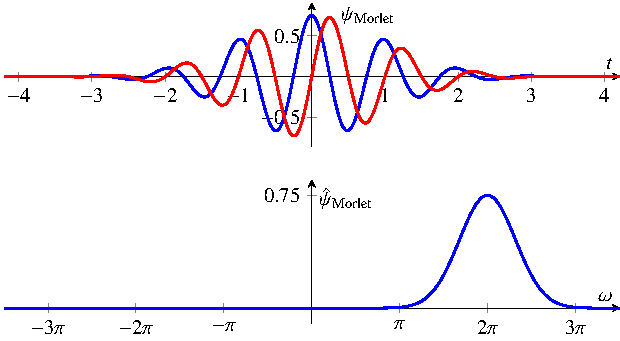
\includegraphics{papers/complex/images/morlet.pdf}
	\caption{Real- (blau) und Imaginärteil (rot) des Morlet-Wavelets für $\sigma = 2\pi$ \label{complex:morlet}}
\end{figure}

In diesem Abschnitt testen wir den Auslöschungsoperator am Gabor-Wavelet.
Wir wechseln in den Fourierbereich und nutzen aus, dass die Fouriertransformierte einer Gauss-Funktion wieder eine Gauss-Funktion ist,
\[
	\Four e^{-\alpha x^2} 
	= \frac{1}{\sqrt{2\alpha}}e^{- \frac{\omega^2}{4\alpha}},
\]
und dass die Multiplikation im Zeitbereich zur Faltung im Frequenzbereich wird.
Zudem verwenden wir die Eulerformel~\eqref{complex:euler}.
Die Fouriertransformierte des Gabor-Wavelet wird hierdurch zu

\begin{equation*}
\begin{aligned}
 \hat{\psi}_\text{Gabor}
 & = \mathcal{F}\Bigg\lbrace c_\sigma e^{-\frac{t^2}{2}}\phantom{\Bigg\rbrace}
 \cdot\; \phantom{\mathcal{F}\Bigg\lbrace}
 \Bigg(\cos\left(\sigma t\right) &&
 &&- \kappa_\sigma\Bigg) \Bigg\rbrace \\
 & = \mathcal{F}\Bigg\lbrace c_\sigma e^{-\frac{t^2}{2}} \Bigg\rbrace 
 *\: \mathcal{F}\Bigg\lbrace\Bigg( \frac12 e^{i\sigma t} &+& \frac12 e^{-i\sigma t}
 &&- \kappa_\sigma \Bigg)\Bigg\rbrace\\
 & = \phantom{\mathcal{F}\Bigg\lbrace} c_\sigma e^{- \frac{\omega^2}{2}} \phantom{\Big\rbrace}
 *\:\phantom{\mathcal{F}\Bigg\lbrace} \Bigg(
  \frac{1}{2}\delta(\omega - \sigma) &-&
  \frac{1}{2}\delta(\omega + \sigma) 
 && - \kappa_\sigma\delta(\omega)
  \Bigg).
\end{aligned}
\end{equation*}

Hierbei bezeichnet $\delta(\omega)$ die Dirac-Distribution.
Hieraus lassen sich die negativen Frequenzen leicht entfernen
\footnote{
	Den Anteil von $\kappa_\sigma$ müsste man genauer betrachten.
	Durch die Faltung mit der Gauss-Funktion entstehen dadurch auch negative Frequenzen.
	Und natürlich besitzt die Exponentialfunktion keinen kompakten Träger, also entstehen auch negative Frequenzen durch die Faltung der Gauss-Funktion mit $\delta(\omega - \sigma)$.
	Wir begnügen uns hier für einmal mit `fast exakt'.
}.
Wir erhalten
\[
	\hat{\psi}^\ast_\text{Gabor} = 
	c_\sigma e^{- \frac{\omega^2}{2}} * (
	\!\sqrt 2 \delta(\omega - \sigma) +
	\frac{1}{\sqrt 2}\kappa_\sigma\delta(\omega) ),
\]
und durch Rücktransformation in den Zeitbereich
\[
	\psi^\ast_\text{Gabor} = c_\sigma e^{- \frac{t^2}{2}} \cdot (\!\sqrt 2 e^{i\sigma t} +	\kappa_\sigma ).
\]
Durch Skalierung der Faktoren $c_\sigma$ und $\kappa_\sigma$ werden wir die Wurzeln los und landen bei einem alten Bekannten: dem Morlet-Wavelet
\[\psi_\text{Morlet} = c_\sigma e^{- \frac{t^2}{2}} \cdot (e^{i\sigma t} + \kappa_\sigma).\]
Wir trafen es bereits in Gleichung~\eqref{cwt:morlet} als Beispiel für die CWT.
Das Morlet-Wavelet ist in Abbildung~\ref{complex:morlet} im Zeit- und Frequenzbereich dargestellt.
Auffallend ist, dass der Realteil bis auf Skalierung unverändert blieb.
Der Operator $\Ana\,$ hat also wie gewünscht das Wavelet nur minimal, respektive gar nicht verändert, sondern lediglich um einen passenden Imaginärteil ergänzt.

Abbildung~\ref{complex:morlet-ex} zeigt die beiden Wavelet-Transformationen unserer Beispiel-Signale mit dem Morlet-Wavelet.
Neu treten alle Farben auf, nicht nur jene für positive und negative Werte.
Zudem sind die Amplituden der Wavelettransformierten, also die Helligkeiten in den Bildern, nun konstant und folgen der Frequenz, statt mit dem Signal mitzuschwingen.
Ansonsten ergeben sich keine Unterschiede zu $\Wave_{\psi_\text{Gabor}}$.

\begin{figure}
	\centering
	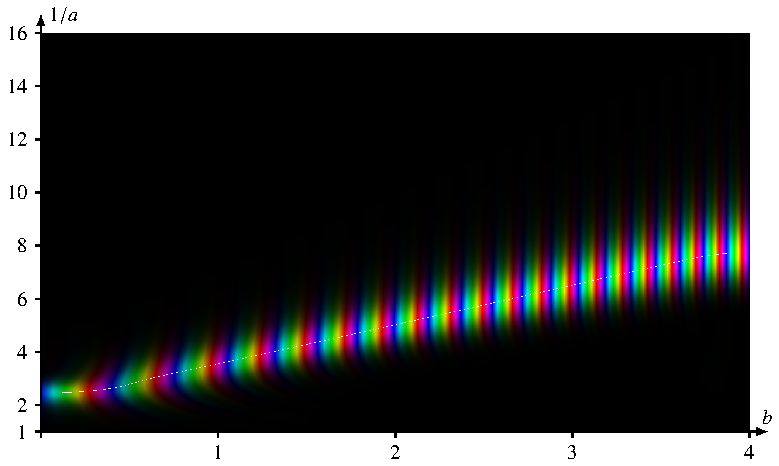
\includegraphics{papers/complex/images/chirp_morlet.pdf}
	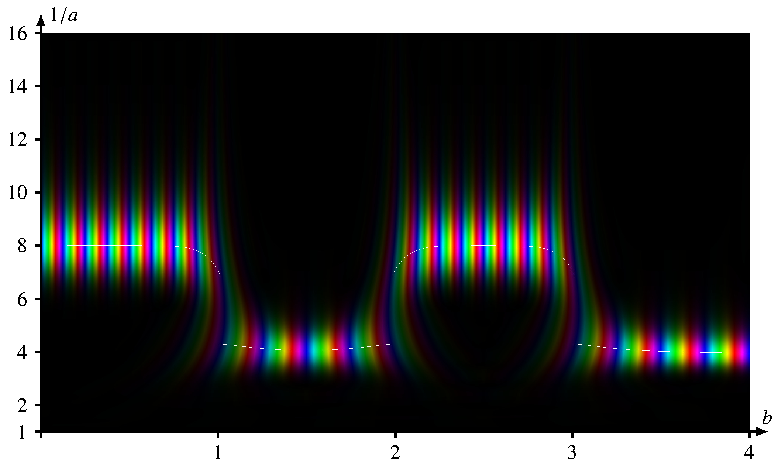
\includegraphics{papers/complex/images/square_morlet.pdf}
	\caption{Wavelet-Transformationen der beiden Beispielsignale mit dem Morlet-Wavelet. 
		Die Oszillation in der Amplitude ist verschwunden.
		Dafür sind die Skalarprodukte nun komplex, es treten alle Farben auf, nicht nur Blau und Gelb.
		Die dominante Frequenz des Morlet-Wavelet ist nahe bei $\omega_\psi \approx 1$. 
		Dadurch entspricht $1/a_\text{max}(b)$ gerade etwa der Momentanfrequenz.
		Allerdings ist die Lokalisierung in der Zeit schlechter als beim Haar-Wavelet.}
	\label{complex:morlet-ex}
\end{figure}
